\chapter{Experimental Evaluation}\label{ch:m-results}

\section{From Communication Regimes to Application Evidence}

The results develop the selection argument in three steps. First, isolated and repeated communication identify candidate stacks and the configurations that make them competitive. Second, a composite CG step tests those candidates alongside computation. Third, aCG determines which observations survive an irregular sparse partition, synchronization dependencies, and convergence. The common-interface results explain what is required to expose these paths through oneCCL.

The principal figures and tables are regenerated from the reconciled archive described in Section~\ref{sec:reproducibility}. Benchmark curves use the median of allocation means with allocation ranges. Solver results first show median completed-trial time for every native path, then retain the reference study's fastest-valid-trial convention as a work-normalized sensitivity view and report MPI variability separately. Lowest point estimates are distinguished from decisive performance differences. Auxiliary configuration controls are identified where their evidence is available only as summaries; the incomplete later NCCL study is confined to Appendix~\ref{app:nccl-preliminary}.

\section{Microbenchmark Results by Communication Pattern}\label{sec:micro-results}

Each pattern is presented with the complete set of measured backends for that campaign, followed immediately by the configuration and execution-contract evidence needed to interpret the curves. The main figures use representative placements; Appendix~\ref{app:complete-results} provides the complete topology panels and the data archive retains every measured size. Comparisons identify complete configured paths rather than attributing a difference to an API or invocation location alone.

\subsection{Ping-Pong: Establishing the Startup Reference}

The first comparison asks whether device-side invocation improves a dependency-ordered exchange. Figure~\ref{fig:m-pingpong-regimes} shows all six measured paths. Across nodes, CUDA MPI has the lowest latency throughout the sweep. At four bytes its allocation-based median is 3.36\,$\mu$s, compared with 7.28\,$\mu$s for OSHMPI, 17.17\,$\mu$s for NVSHMEM, and 28.78\,$\mu$s for NCCL. Device invocation therefore does not remove the startup advantage of the evaluated MPI path.

\begin{figure}[htbp]
\centering
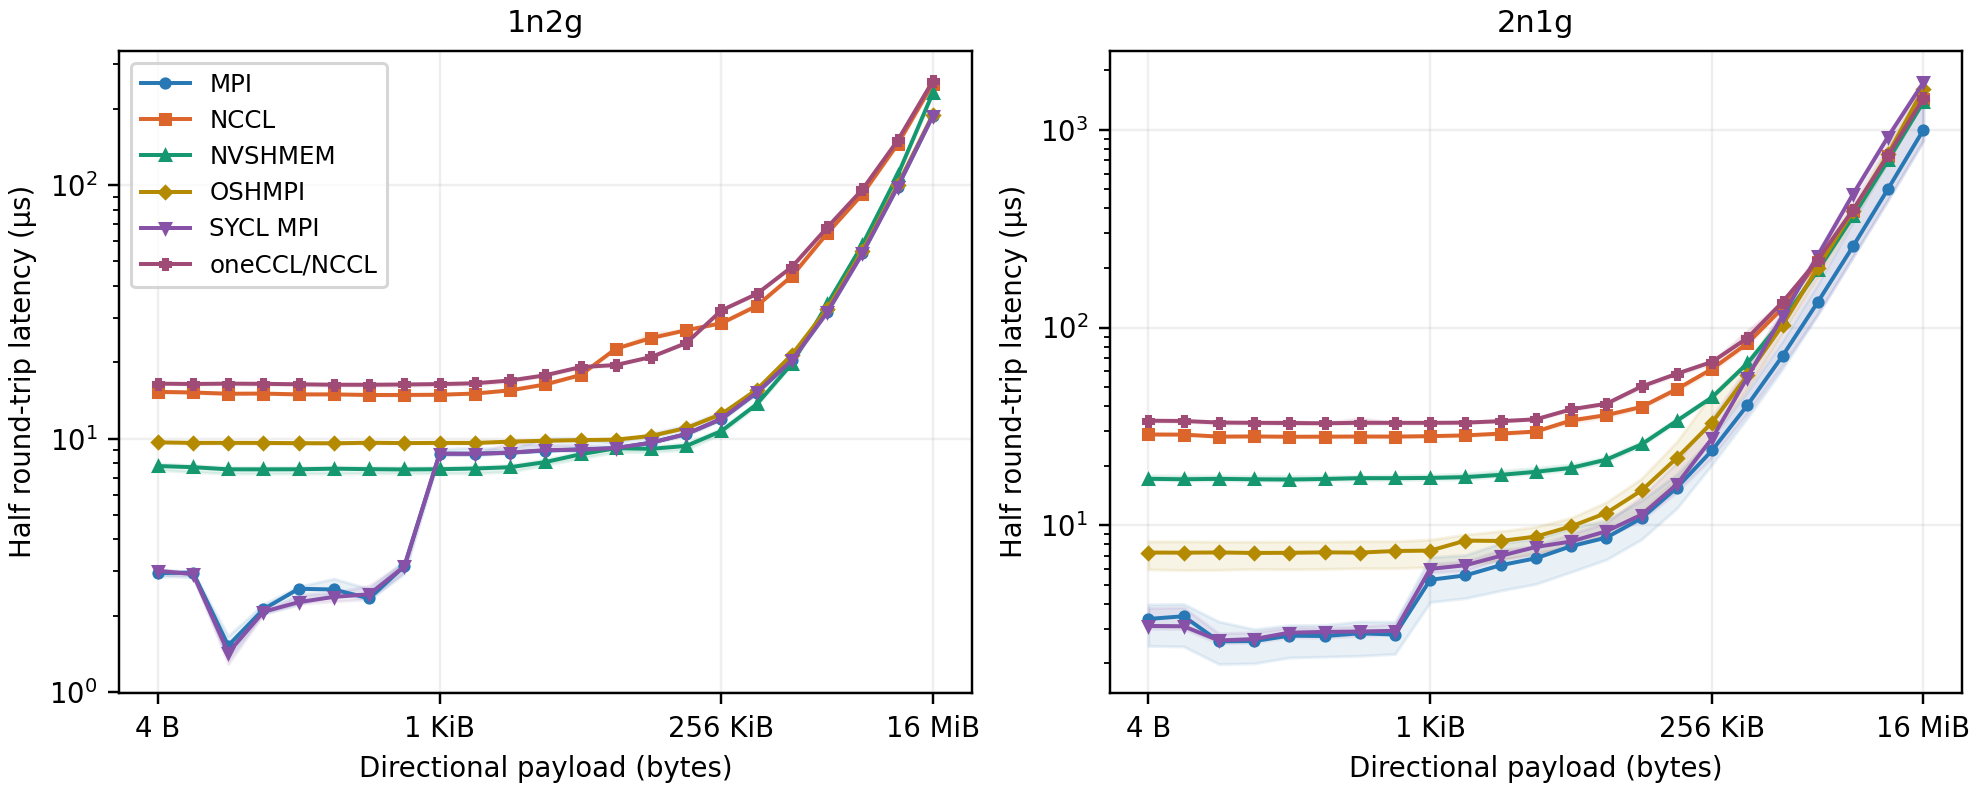
\includegraphics[width=\textwidth]{figures/results/pingpong-regimes.png}
\caption{Ping-pong latency for all six measured stacks within one node and across two nodes. Points are medians of five allocation means; shading spans those means. Latency is half the round-trip time.}
\label{fig:m-pingpong-regimes}
\end{figure}

\begin{table}[htbp]
\centering
\caption{Inter-node ping-pong latency on \texttt{2n1g}, including SYCL paths. Values are allocation-based medians in \,$\mu$s.}
\label{tab:m-pingpong-inter}
\footnotesize
% Generated by tools/rebuild_main_evidence.py; include outside tabular.
\begin{tabular}{lrr}
\toprule
Stack & 4\,B & 16\,MiB\\
\midrule
MPI & 3.358 & 1000.370\\
SYCL MPI & 3.094 & 1736.543\\
OSHMPI & 7.275 & 1614.043\\
NVSHMEM & 17.171 & 1388.240\\
NCCL & 28.781 & 1436.673\\
oneCCL/NCCL & 33.789 & 1444.770\\
\bottomrule
\end{tabular}

\end{table}

Within a node, NVSHMEM becomes competitive over an intermediate message range, while MPI again improves relative to it at large payloads. Table~\ref{tab:m-pingpong-inter} also shows that CUDA and SYCL MPI cannot be assumed to agree at every size: their small-message results are close to the MPI startup regime, but their large-message endpoints differ substantially. A shared MPI installation supplies a useful comparison, not a guarantee of identical execution costs.

The common-interface NCCL path is also visible in this startup-sensitive pattern. At four-byte inter-node ping-pong, oneCCL/NCCL takes 33.8\,$\mu$s against 28.8\,$\mu$s for direct NCCL, approximately 17\% more. This changes the compute interface and orchestration as well as the adapter call, so it measures the complete oneCCL/NCCL stack rather than isolated wrapper overhead. The ping-pong result is consequently a small-message half-round-trip comparison, not an estimate of an initiation-only launch saving.

\subsection{Halo: Repetition Changes the Trade-off}

A repeated neighbor exchange offers a different opportunity from ping-pong. The fixed submission and completion cost can be spread across many exchanges, while multiple peer transfers can proceed together. Figure~\ref{fig:m-halo-regimes} contrasts isolated and steady-state execution on one and eight nodes.

\begin{figure}[htbp]
\centering
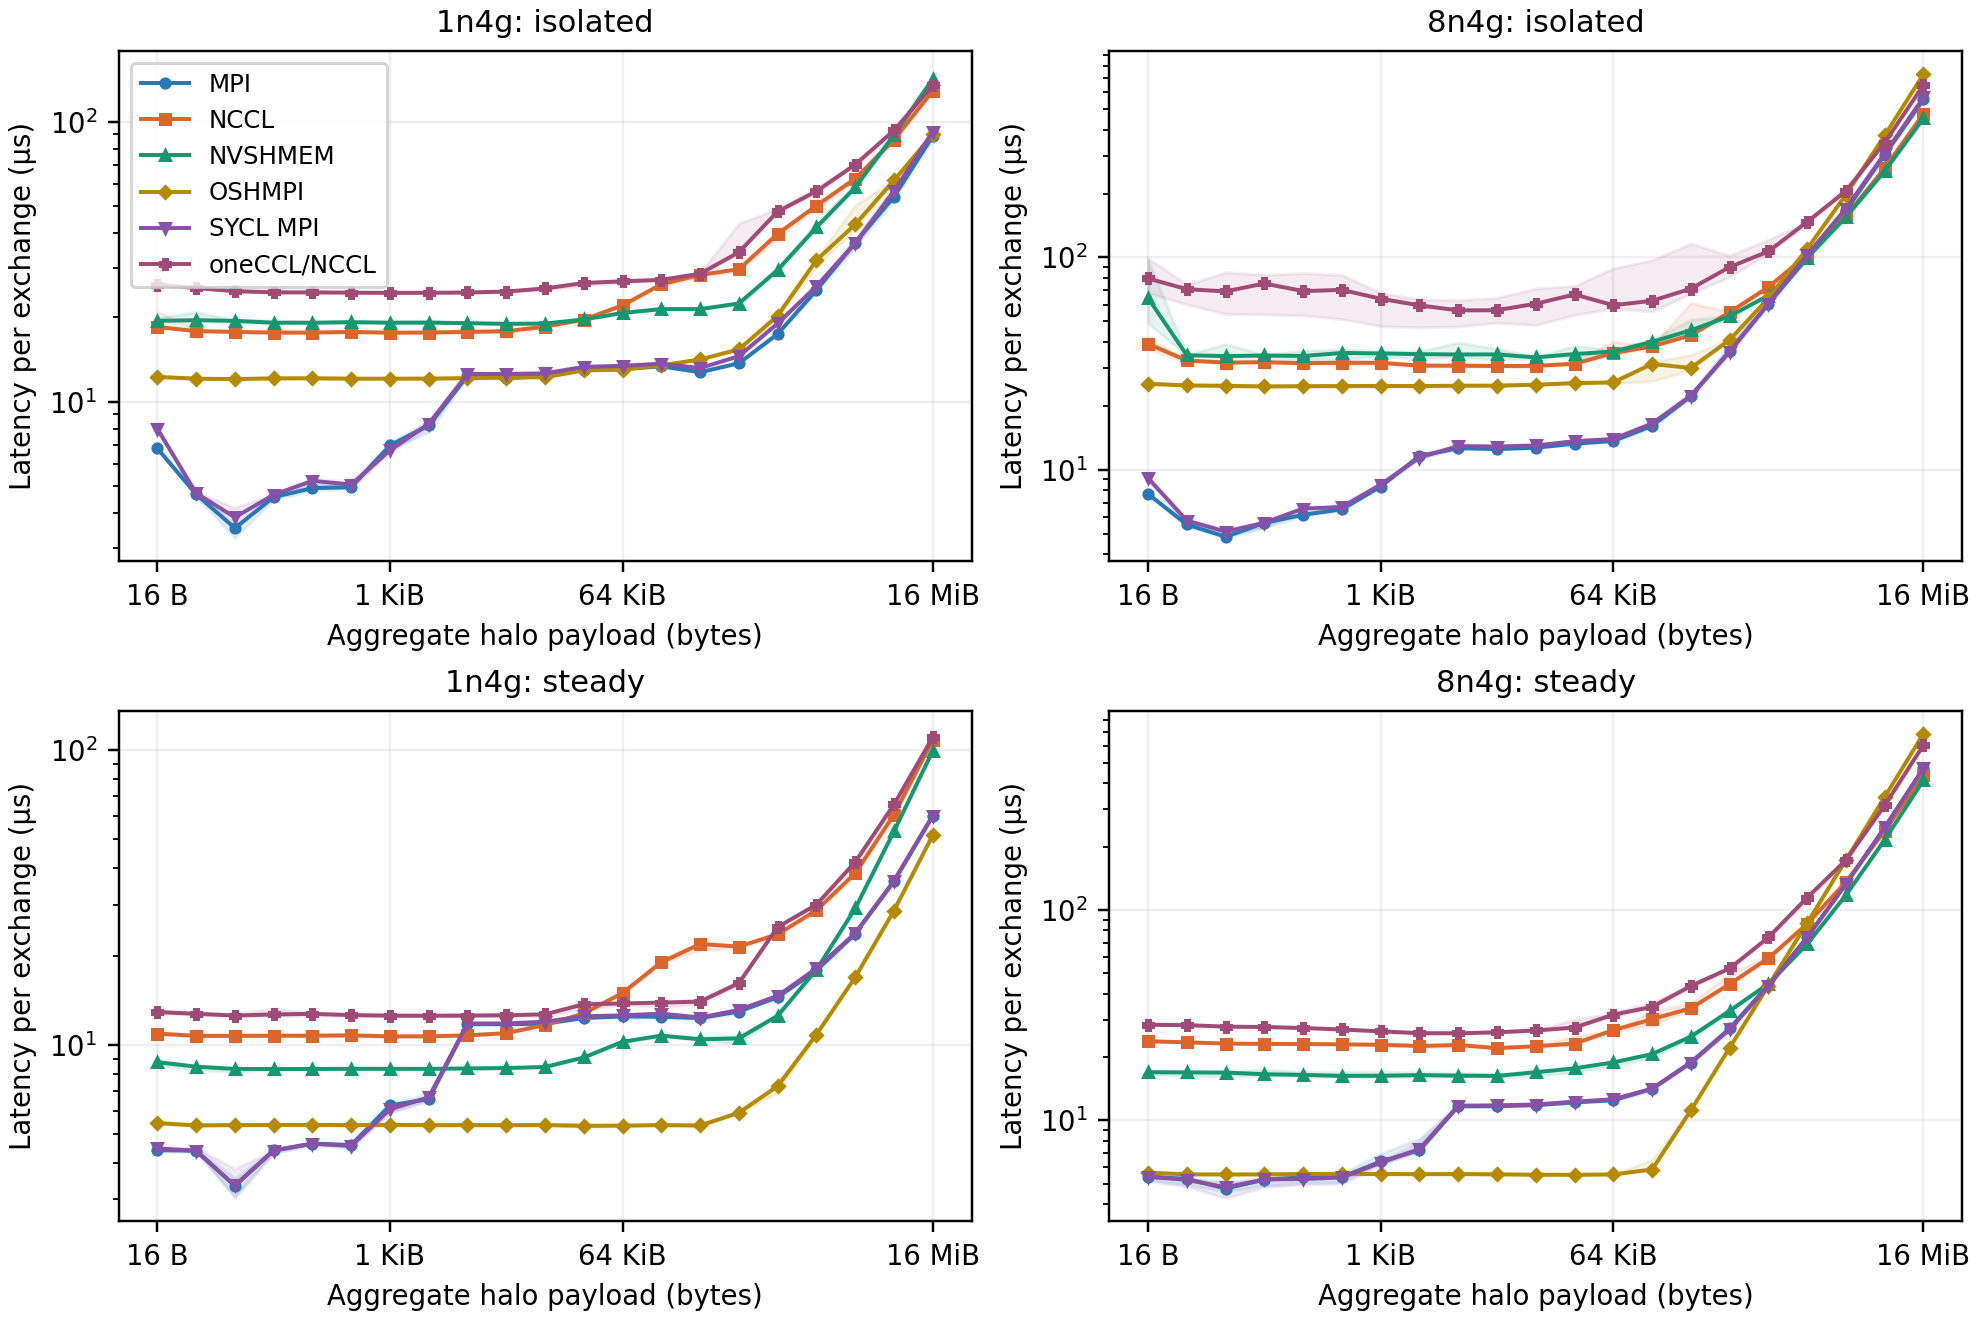
\includegraphics[width=\textwidth]{figures/results/halo-regimes.png}
\caption{Isolated and steady-state halo latency for all six measured stacks. Steady-state values amortize a batch of 100 exchanges. Points and shading show allocation medians and ranges; payload counts two sends and two receives.}
\label{fig:m-halo-regimes}
\end{figure}

MPI supplies the low-startup reference for isolated exchanges. Batching makes OSHMPI competitive across small and intermediate payloads because its batch-level completion cost is amortized. At large multi-node payloads, persistent NVSHMEM sustains the highest rate among the direct paths in Table~\ref{tab:m-halo-bandwidth}. Its approximately 41\,GB/s aggregate rate remains similar from two to eight nodes, while MPI reaches approximately 34--36\,GB/s.

\begin{table}[htbp]
\centering
\caption{Peak steady-state halo bandwidth computed from allocation-median latency, in GB/s. The numerator is aggregate logical halo volume, not one NIC's traffic.}
\label{tab:m-halo-bandwidth}
\input{data/main-campaign/halo_1d-bandwidth-table.tex}
\end{table}

The favorable regime for the persistent, kernel-invoked NVSHMEM path is thus sustained neighbor work rather than universally low latency. The SYCL MPI and oneCCL/NCCL curves further show that portable submission paths do not remove the same isolated-versus-steady distinction. This supports persistent execution as a candidate explanation in RQ1, while the host-driven OSHMPI result shows that batching and completion policy also matter independently of invocation location. Because the paths differ in signaling, persistence, sampling, and progress, these measurements do not isolate a launch-overhead saving by themselves. The inter-node NVSHMEM result specifically describes device invocation with CPU-proxy-assisted \texttt{ibrc} progress.

\subsection{Allreduce: Configuration and Payload Both Matter}

For reductions, the dominant distinction is between startup-sensitive scalar work and bulk combination. Figure~\ref{fig:m-allreduce-backends} shows all seven measured paths at representative intra- and multi-node placements. NCCL-based paths lead the large-message regime (Table~\ref{tab:m-allreduce-bandwidth}). NVSHMEM normally dispatches these benchmark collectives through NCCL, so their similar throughput is evidence about that configured path rather than two independent collective algorithms.

\begin{figure}[htbp]
\centering
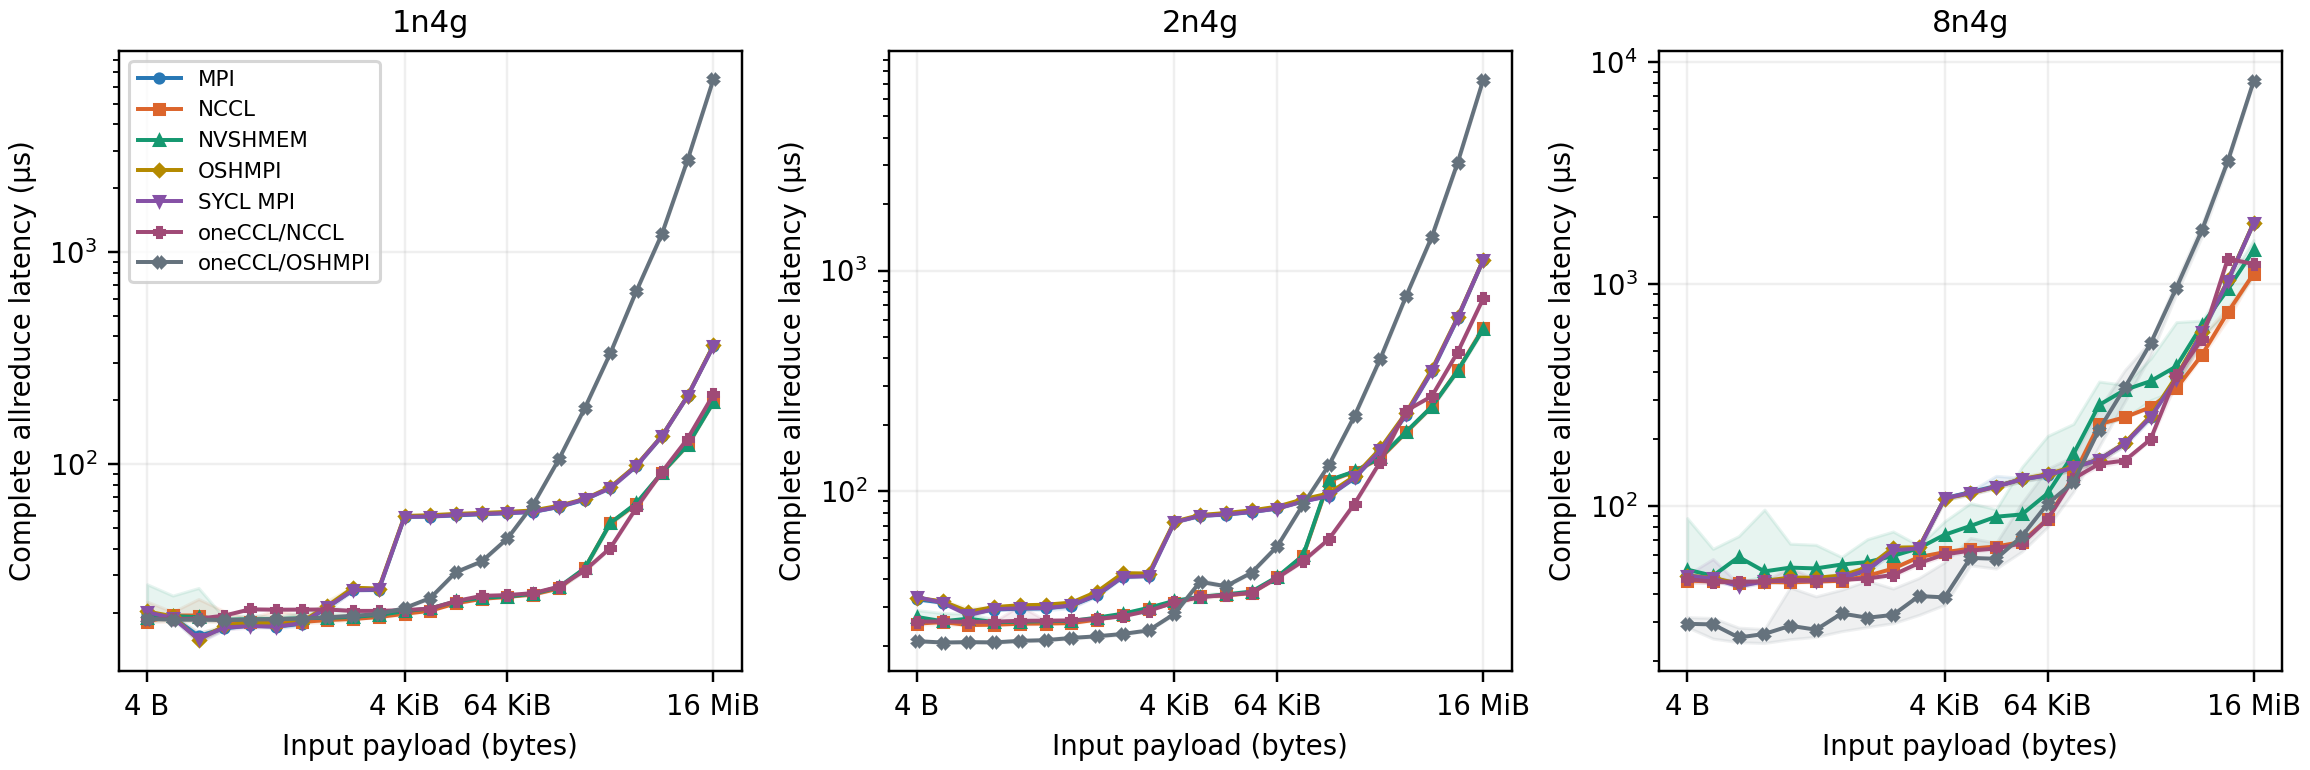
\includegraphics[width=\textwidth]{figures/results/allreduce-backends.png}
\caption{Allreduce latency for all seven measured stacks at representative placements. Points are medians of allocation means and shading spans those means. The input payload is per rank; the single-rank control is discussed separately.}
\label{fig:m-allreduce-backends}
\end{figure}

\begin{table}[htbp]
\centering
\caption{Peak allreduce bus bandwidth in GB/s, recomputed as input bytes divided by allocation-median latency and multiplied by $2(P-1)/P$.}
\label{tab:m-allreduce-bandwidth}
% Generated by tools/rebuild_main_evidence.py; include outside tabular.
\begin{tabular}{lrrr}
\toprule
Topology & CUDA NCCL & CUDA NVSHMEM & CUDA MPI\\
\midrule
\texttt{1n4g} & 127.5 & 128.3 & 69.7\\
\texttt{2n4g} & 51.8 & 53.9 & 26.3\\
\texttt{4n4g} & 31.8 & 14.3 & 19.9\\
\texttt{8n4g} & 29.5 & 11.9 & 17.3\\
\bottomrule
\end{tabular}

\end{table}

The UCC control explains why MPI's result cannot be summarized by a single library label. Figure~\ref{fig:m-ucc-allreduce} shows a size-dependent trade-off. UCC improves large reductions, but incurs penalties in part of the small-message range. The exceptions include an intra-node region around 4\,KiB; its benefit is not uniform even on one node. On the larger multi-node configurations, the crossover back to a benefit occurs around 64\,KiB.

\begin{figure}[htbp]
\centering
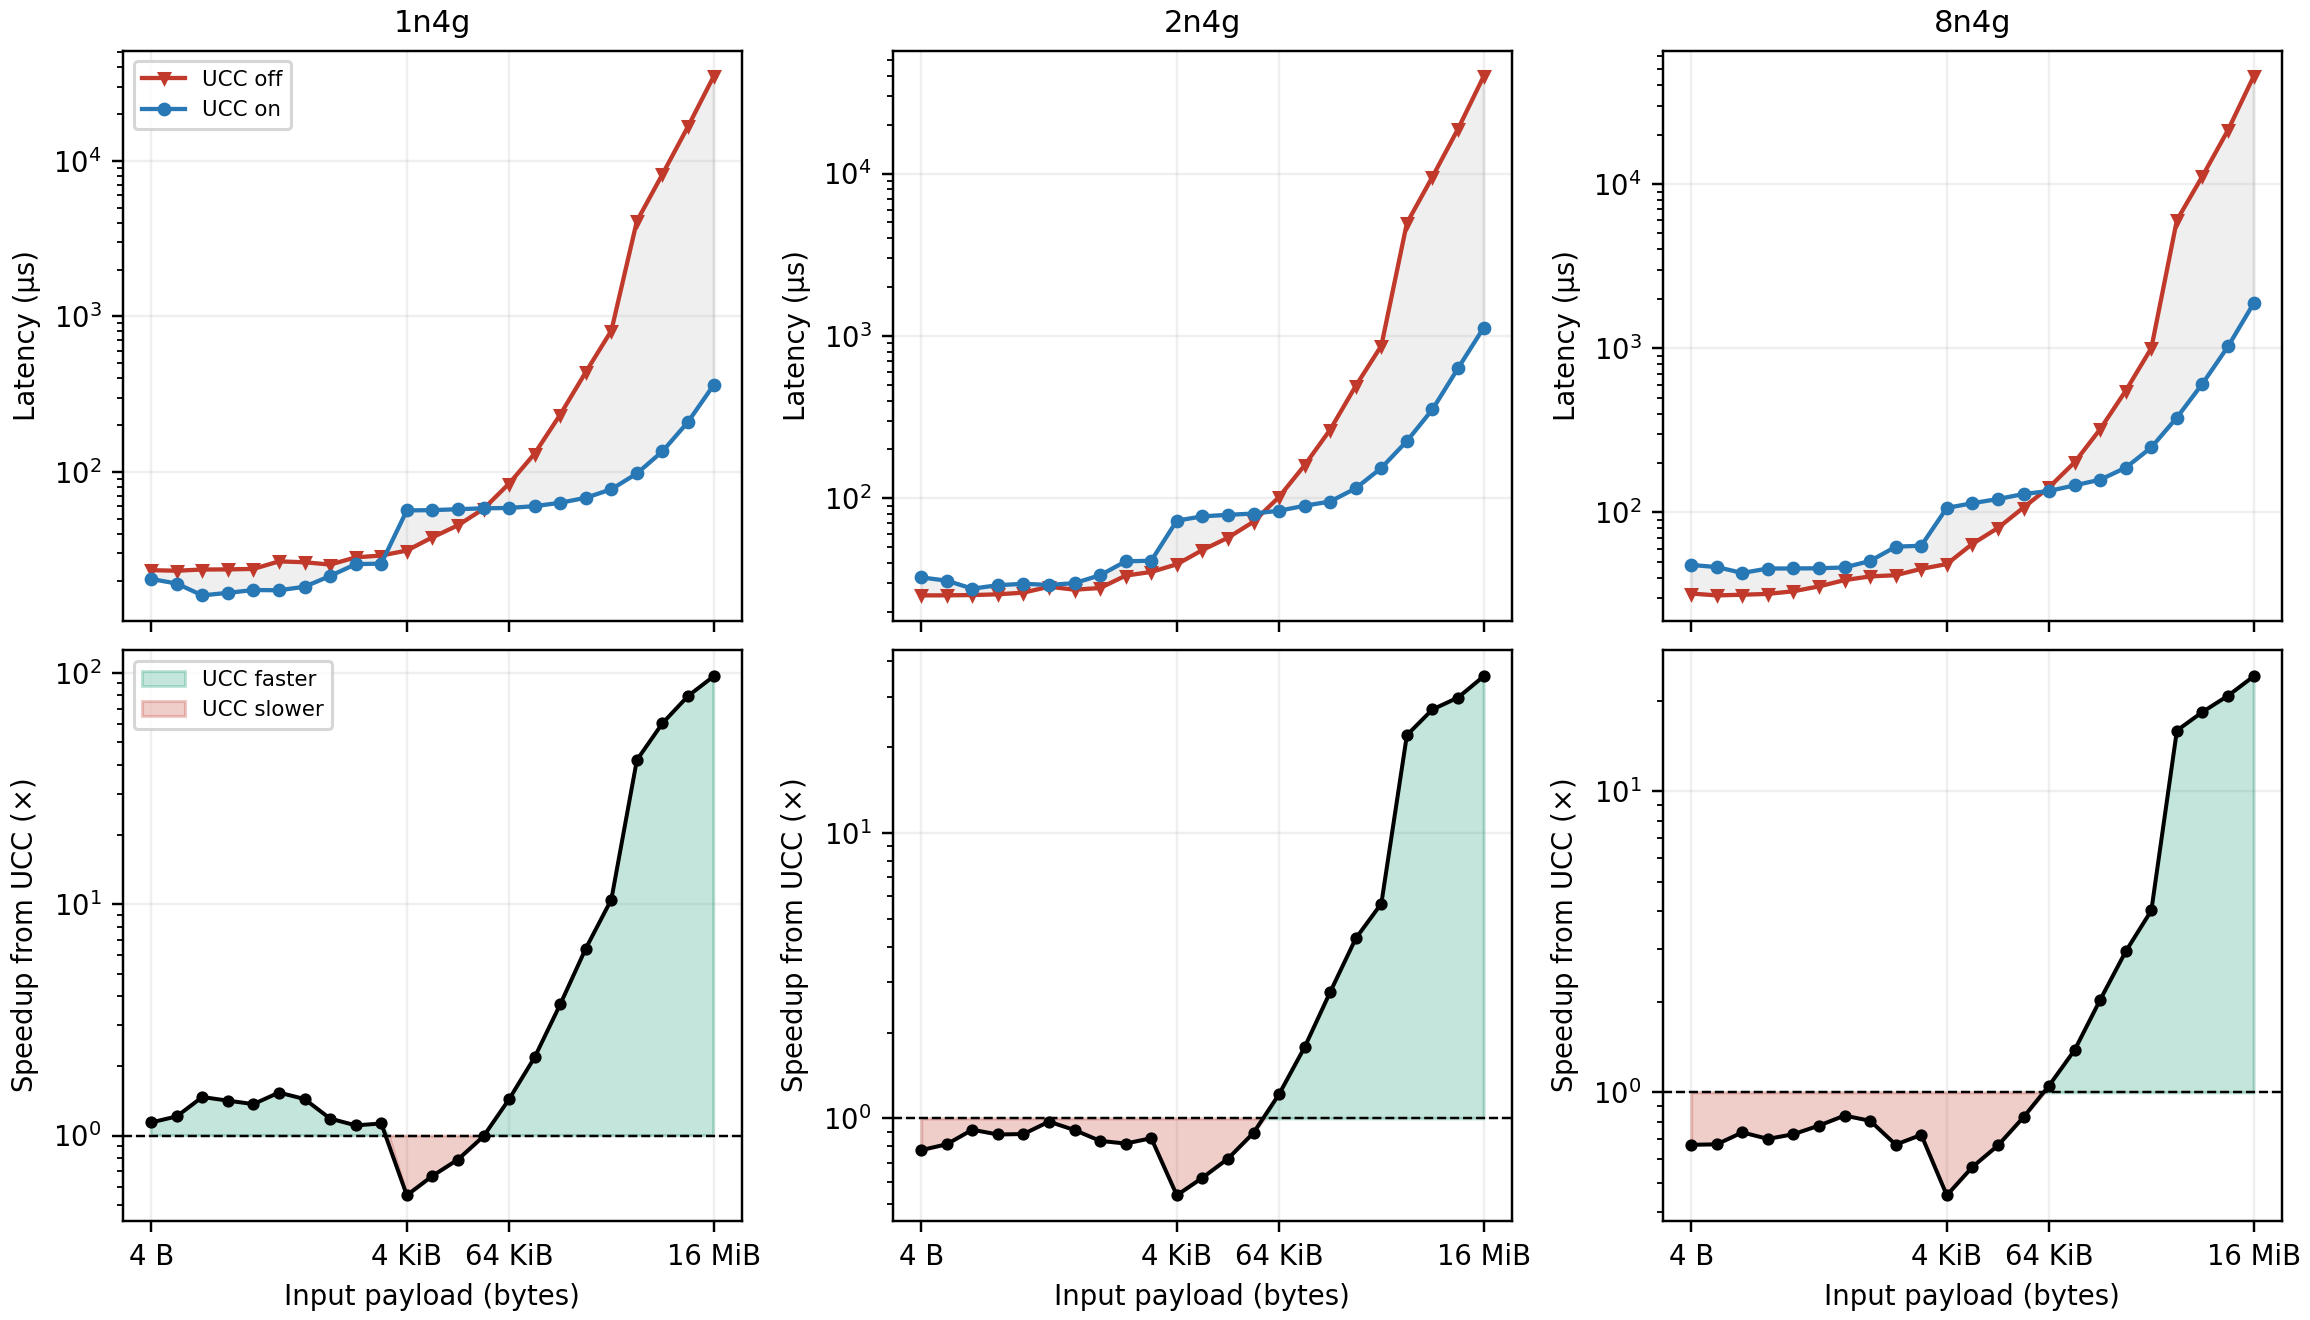
\includegraphics[width=\textwidth]{figures/results/ucc-ab-allreduce.png}
\caption{Paired UCC allreduce summary means. Ratios above one favor UCC. Selected topologies show both the intra-node exception and multi-node crossover. The SYCL \texttt{8n4g} series is absent because no matched pair was retained.}
\label{fig:m-ucc-allreduce}
\end{figure}

The discontinuity near 4\,KiB is consistent with the UCC TL/UCP source's change from a latency-oriented recursive k-nomial schedule to scatter-reduce/allgather k-nomial \cite{openucx_ucc_source_2026}. Source defaults explain a plausible mechanism, while forcing alternatives or recording the exact selected schedule would strengthen attribution for individual cells. The experiment uses one fixed UCC policy for the standalone allreduce sweep, so it does not claim a pointwise optimal configuration.

The single-rank allreduce control is anomalously slow for large buffers: the auxiliary UCC data report approximately 21\,ms at 16\,MiB, despite no inter-rank reduction. It is excluded as a reference for network startup. A one-rank control removes network communication, but can still expose internal copies or reduction implementation costs.

The complete backend view also exposes the cost of oneCCL/OSHMPI's symmetric staging. On \texttt{1n4g}, the four-byte allreduce medians are 20.3\,$\mu$s directly and 18.7\,$\mu$s through oneCCL/OSHMPI. At 16\,MiB, they are 364\,$\mu$s and 6509\,$\mu$s, respectively: the adapted path is approximately 18 times slower. The direct device-resident reduction and symmetric-staging adapter use different memory and completion paths. The comparison therefore identifies the cost of the evaluated integration choice, not an intrinsic penalty of the oneCCL API.

This pattern demonstrates why functional interface compatibility and performance retention must be evaluated separately. The OSHMPI adapter waits for queue dependencies, stages ordinary operands through symmetric storage, performs a blocking host operation, and returns an already-complete event. Those semantics preserve correctness but remove the asynchronous opportunity retained by the NCCL path.

\subsection{All-to-All: Correct the Default Before Ranking Libraries}

All-to-all gives the clearest example of a configuration changing the apparent library ranking. Figure~\ref{fig:m-alltoall-backends} first shows all seven measured stacks against bytes per peer, rather than the topology-dependent aggregate send-buffer size. The MPI default changes regime sharply as rank count and per-peer size increase, while oneCCL/OSHMPI's staged path remains substantially more expensive. In the paired UCC summaries, the non-UCC MPI path takes hundreds of microseconds for tiny per-peer payloads at 16 and 32 ranks. Enabling UCC reduces these costs by approximately 17--34 times. Figure~\ref{fig:m-ucc-alltoall} shows that this gain is concentrated in the high-rank, small-message region; larger payloads can instead favor the non-UCC configuration.

\begin{figure}[htbp]
\centering
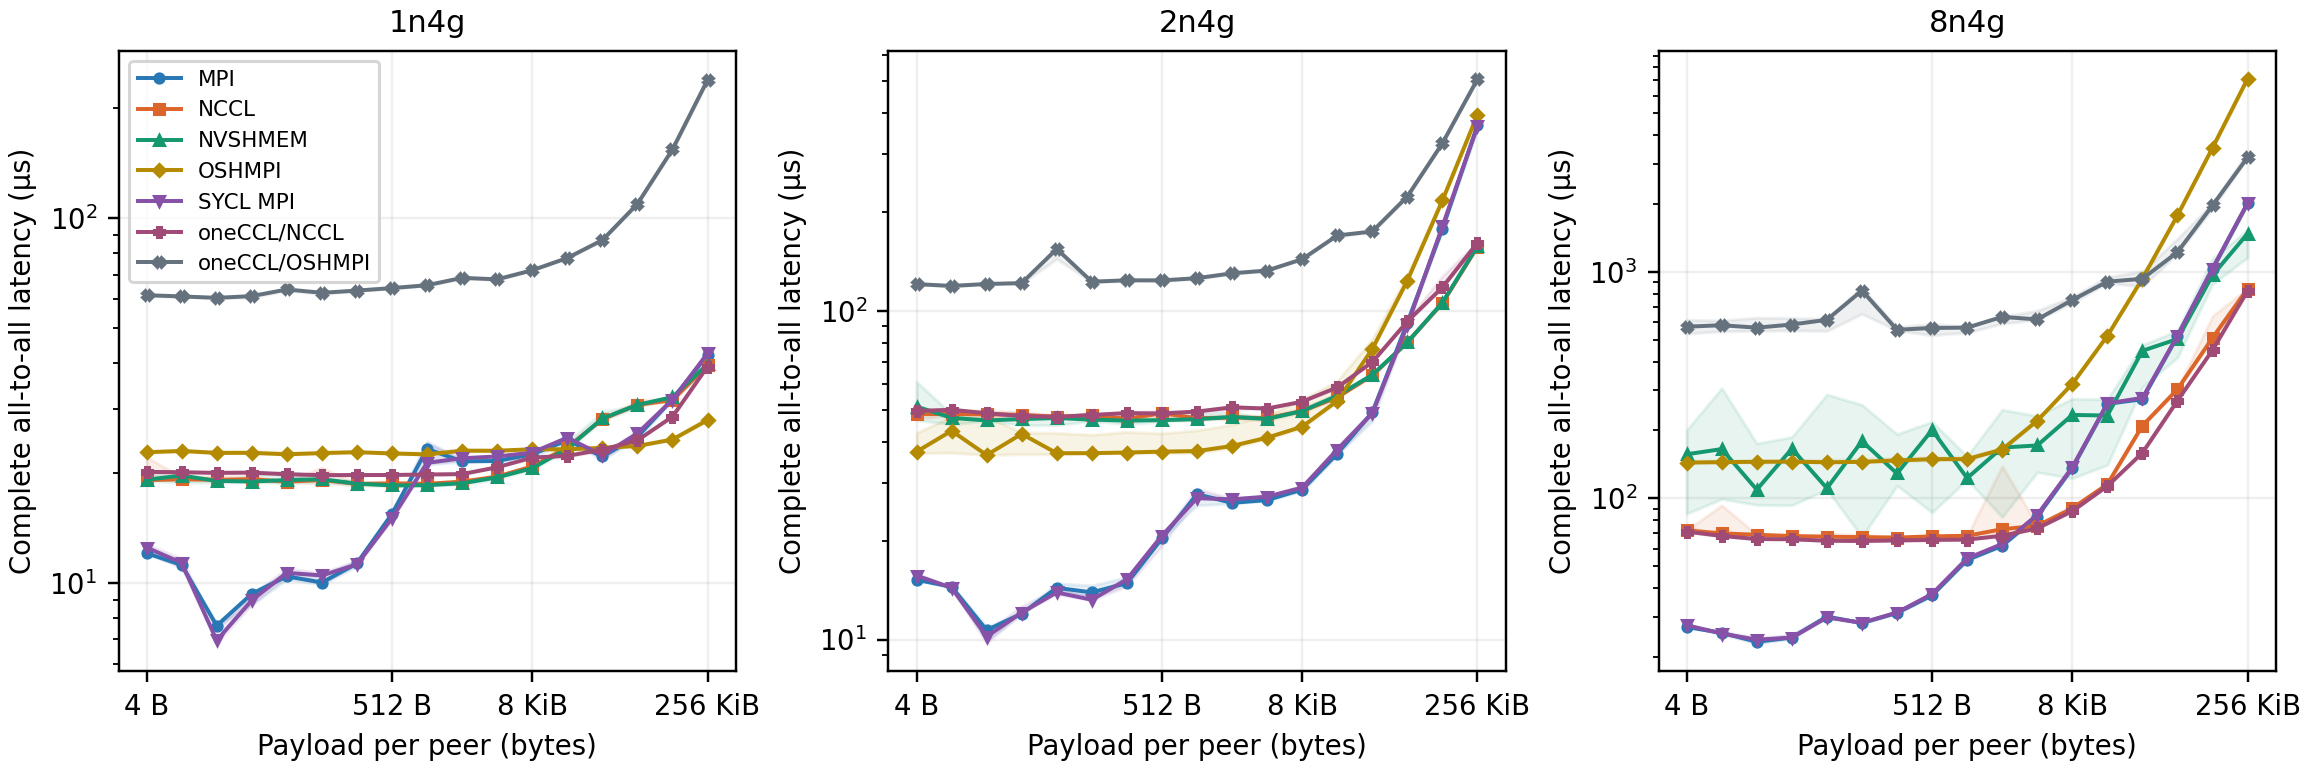
\includegraphics[width=\textwidth]{figures/results/alltoall-backends.png}
\caption{All-to-all latency for all seven measured stacks at representative placements. The horizontal axis is payload per peer; points are medians of allocation means and shading spans those means.}
\label{fig:m-alltoall-backends}
\end{figure}

\begin{figure}[htbp]
\centering
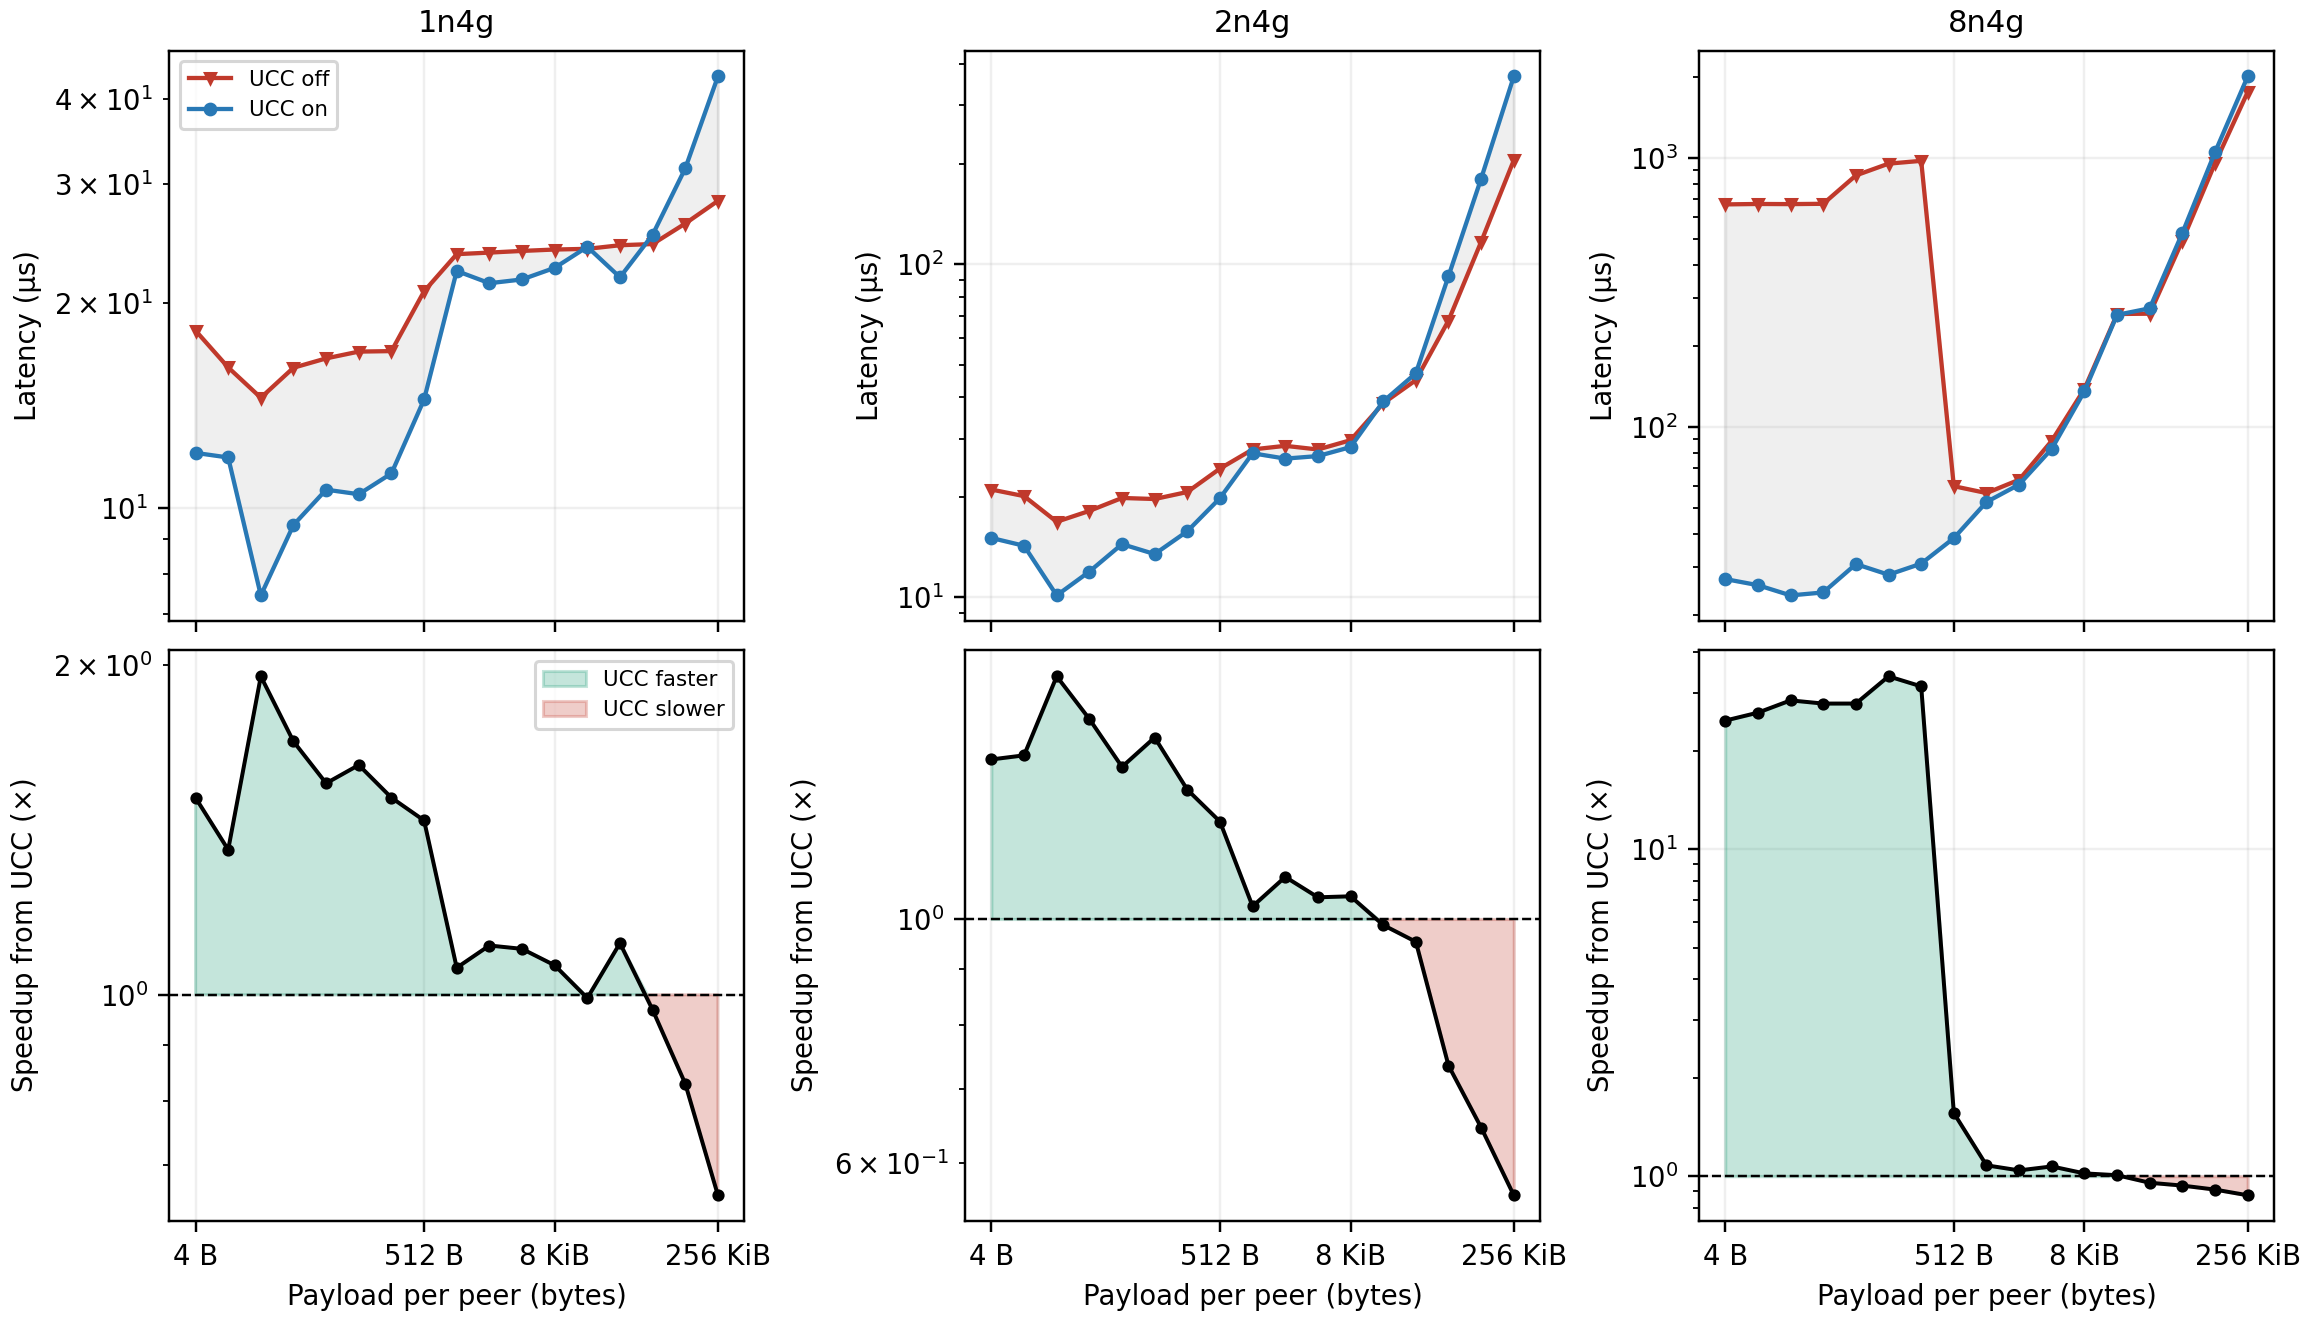
\includegraphics[width=\textwidth]{figures/results/ucc-ab-alltoall.png}
\caption{Paired UCC all-to-all summary means. The payload axis is bytes per peer. The large high-rank benefit and the smaller large-message penalty motivate treating configuration as part of stack selection.}
\label{fig:m-ucc-alltoall}
\end{figure}

An auxiliary forced-algorithm control isolates the problematic default (Table~\ref{tab:m-alltoall-forced}). Below 512 bytes per peer, the default follows modified Bruck; forcing linear or synchronized-linear exchange avoids most of the penalty. This supports an algorithm-selection explanation rather than attributing the full gain to a uniquely efficient UCC network transport.

\begin{table}[htbp]
\centering
\caption{Auxiliary forced Open MPI all-to-all control at 16 ranks, UCC disabled, in \,$\mu$s. Values are retained from the configuration-analysis record.}
\label{tab:m-alltoall-forced}
\scriptsize
\begin{tabular}{rrrrrr}
\toprule
B/peer & Linear & Pairwise & Modified Bruck & Linear sync & Default\\
\midrule
4 & 25.7 & 64.8 & 340.0 & 29.9 & 342.3\\
16 & 22.1 & 58.1 & 341.4 & 24.5 & 341.2\\
256 & 27.9 & 72.4 & 421.2 & 29.6 & 420.0\\
512 & 31.7 & 79.6 & 429.2 & 34.9 & 38.8\\
\bottomrule
\end{tabular}
\end{table}

Modified Bruck reduces communication rounds by forwarding data, but the Open MPI implementation also rotates buffers, constructs indexed datatypes, and copies noncontiguous blocks \cite{bruck_alltoall_1997,openmpi_alltoall_source_2026}. Those local operations can be expensive on GPU-resident buffers. The UCC dispatch trace identifies its UCP transport layer, whose CUDA default uses contiguous peer slices and nonblocking tagged communication \cite{venkata_ucc_2024,openucx_ucc_source_2026}. This explains the structural difference; it does not replace a profile of individual copy costs.

At large payloads, NCCL-based paths regain the advantage. Table~\ref{tab:m-alltoall-bandwidth} gives the endpoint at 256\,KiB per peer. The closely spaced direct-NCCL and oneCCL/NCCL results should be read against allocation variation. The all-to-all archive combines measurement rounds, so it establishes the large regime differences more securely than small cross-backend margins.

\begin{table}[htbp]
\centering
\caption{All-to-all aggregate bandwidth at 256\,KiB per peer, in GB/s. The numerator includes each rank's self block.}
\label{tab:m-alltoall-bandwidth}
\footnotesize
% Generated by tools/rebuild_main_evidence.py; include outside tabular.
\begin{tabular}{lrrrr}
\toprule
Topology & CUDA MPI & CUDA NCCL & CUDA NVSHMEM & oneCCL/NCCL\\
\midrule
\texttt{2n4g} & 5.7 & 13.4 & 13.3 & 13.0\\
\texttt{4n4g} & 4.4 & 10.3 & 8.2 & 10.5\\
\texttt{8n4g} & 4.2 & 10.0 & 5.7 & 10.2\\
\bottomrule
\end{tabular}

\end{table}

At the largest \texttt{8n4g} payload, direct NCCL and oneCCL/NCCL are within approximately 2\%. The adapter and SYCL orchestration are therefore much less visible at this bulk endpoint than in four-byte ping-pong. This is again a complete-stack comparison, not an isolated adapter measurement. Together with the staged oneCCL/OSHMPI curve, it shows that a common interface can retain a backend's bulk regime when it preserves its asynchronous data path, while a blocking staging strategy can change the regime entirely.

These primitive results leave several plausible candidates: MPI for startup-sensitive transfers, persistent NVSHMEM for large repeated halos, and NCCL-based paths for bulk collectives. The next question is whether composing operations preserves those advantages.

\section{Composition in the \texttt{cg\_step} Benchmark}\label{sec:cg-step-results}

\subsection{Communication--Computation Sequence}

The composite archive covers seven placements, five global grid sides, and six backends, with nine successful trials per cell. It preserves a halo--stencil--reduction sequence but not the complete CG recurrence: the two reduced scalars are terminal outputs and do not gate a dependent GPU update. Table~\ref{tab:m-cg-step} reports the lowest allocation-median estimate under that contract. OSHMPI leads 25 of the 30 multi-rank cells, including all multi-node placements; NCCL leads the remaining five intra-node cells. The single-GPU NCCL-labeled implementation leads its controls, where the result reflects local execution and synchronization rather than network performance.

\begin{table}[htbp]
\centering
\caption{Lowest allocation-median \texttt{cg\_step} time by placement and global grid side. This is a point-estimate ranking for the synthetic sequence, not a significance test or a solver-ready ranking.}
\label{tab:m-cg-step}
\footnotesize
% Generated by tools/rebuild_main_evidence.py; include outside tabular.
\begin{tabular}{lccccc}
\toprule
Topology & 512 & 1024 & 2048 & 4096 & 8192\\
\midrule
\texttt{1n1g} & NCCL & NCCL & NCCL & NCCL & NCCL\\
\texttt{1n2g} & NCCL & NCCL & NCCL & OSHMPI & OSHMPI\\
\texttt{1n4g} & OSHMPI & NCCL & NCCL & OSHMPI & OSHMPI\\
\texttt{2n1g} & OSHMPI & OSHMPI & OSHMPI & OSHMPI & OSHMPI\\
\texttt{2n4g} & OSHMPI & OSHMPI & OSHMPI & OSHMPI & OSHMPI\\
\texttt{4n4g} & OSHMPI & OSHMPI & OSHMPI & OSHMPI & OSHMPI\\
\texttt{8n4g} & OSHMPI & OSHMPI & OSHMPI & OSHMPI & OSHMPI\\
\bottomrule
\end{tabular}

\end{table}

\begin{figure}[htbp]
\centering
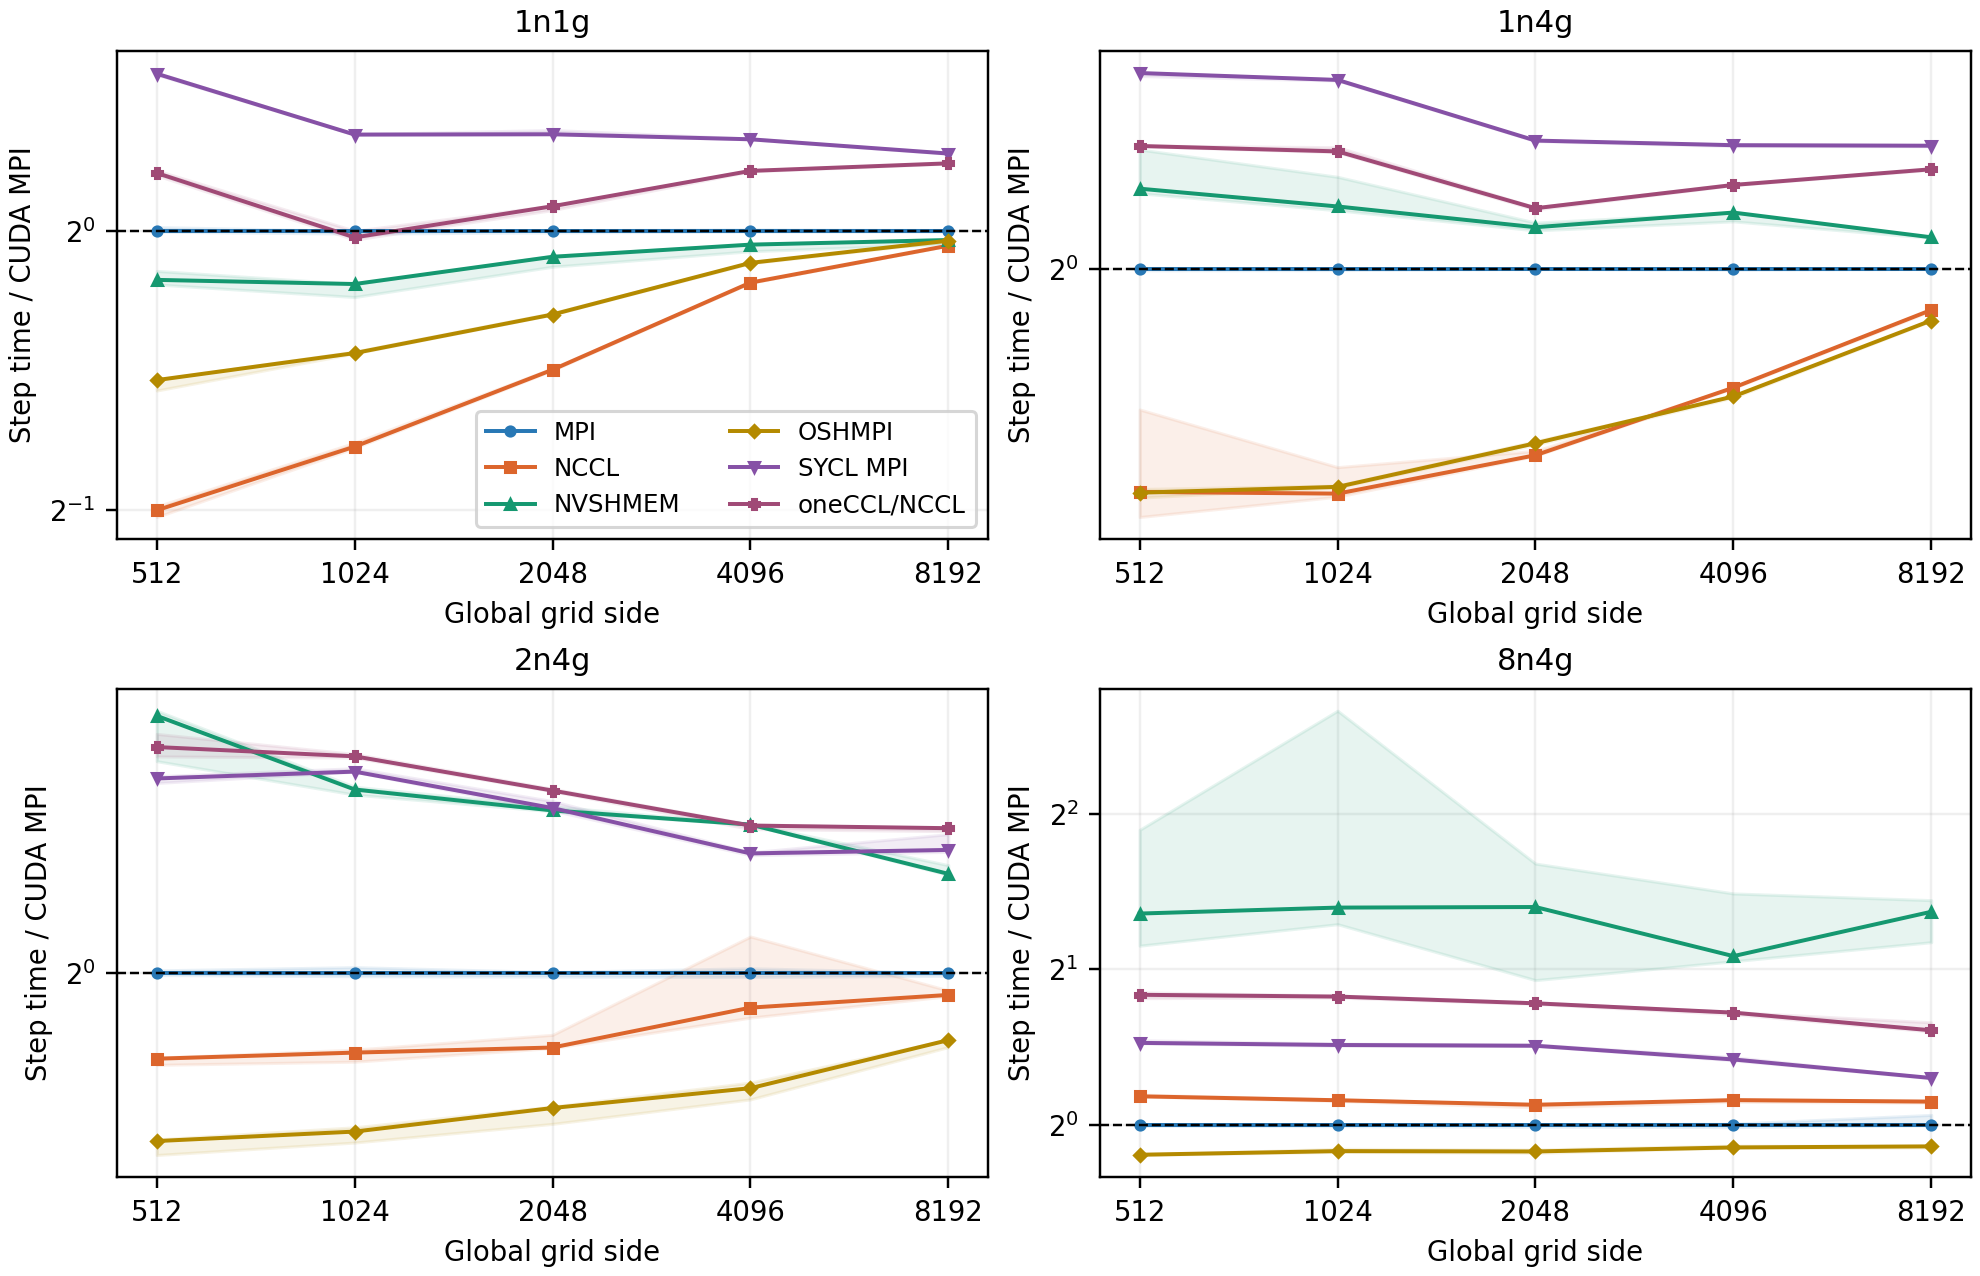
\includegraphics[width=\textwidth]{figures/results/cg-step-relative.png}
\caption{Composite-step time relative to CUDA MPI at the same global grid side and placement. Centers are allocation medians; bands are allocation ranges divided by the fixed reference median, not confidence intervals for the ratio. Values below one favor the compared stack.}
\label{fig:m-cg-relative}
\end{figure}

Figure~\ref{fig:m-cg-relative} shows why the margin matters. The direct CUDA paths approach one another as single-GPU work grows. At larger rank counts, communication and orchestration remain visible, and NVSHMEM exhibits substantial allocation variation. Some intra-node NCCL and OSHMPI estimates are close enough that assigning a categorical winner overstates the evidence.

The OSHMPI result also needs an execution-contract qualification: its archived scalar path ends with the reduction result in host memory. It avoids the return copy and consumer dependency present in a solver. The result identifies an efficient implementation of this synthetic step, not yet an efficient end-to-end CG reduction path.

\subsection{Phase Diagnostics}

Table~\ref{tab:m-cg-phases} uses the separate synchronized phase pass at \texttt{4n4g}, side 512. The OSHMPI reduction phase is smaller than the corresponding MPI and NCCL phases, while NVSHMEM's halo and reduction costs contribute to its larger total. The SYCL paths also expose additional computation and runtime costs.

\begin{table}[htbp]
\centering
\caption{Archived mean \texttt{cg\_step} phase costs on \texttt{4n4g}, side 512, in \,$\mu$s. Step is the unsplit mean; gap is phase sum minus step.}
\label{tab:m-cg-phases}
\scriptsize
% Generated by tools/rebuild_main_evidence.py; include outside tabular.
\begin{tabular}{lrrrrrrr}
\toprule
Backend & Pack & Halo & Compute & Reduce & Sum & Step & Gap\\
\midrule
MPI & 13.3 & 23.7 & 24.6 & 58.7 & 120.3 & 111.3 & 9.0\\
NCCL & 28.5 & 38.6 & 23.0 & 76.3 & 166.3 & 107.7 & 58.6\\
NVSHMEM & 14.3 & 77.6 & 35.6 & 125.4 & 252.8 & 215.5 & 37.3\\
OSHMPI & 13.5 & 25.3 & 24.4 & 37.7 & 100.9 & 88.9 & 12.0\\
SYCL MPI & 11.3 & 25.2 & 67.6 & 62.3 & 166.4 & 164.0 & 2.4\\
oneCCL/NCCL & 11.7 & 48.8 & 45.7 & 107.4 & 213.6 & 183.0 & 30.6\\
\bottomrule
\end{tabular}

\end{table}

For NCCL, the phase sum is approximately 166.3\,$\mu$s and the unsplit mean 107.7\,$\mu$s. Their 58.6\,$\mu$s difference is about 35\% of the phase sum, or 54\% of the unsplit time. The denominator changes the percentage. More importantly, the gap includes synchronization introduced by instrumentation and variation between passes; it cannot be reported as a measured overlap fraction.

\subsection{Scalar Placement: An Advantage with an Unmatched Boundary}

The auxiliary OSHMPI placement control compares host-staged reductions with CUDA symmetric operands and UCC enabled (Table~\ref{tab:m-oshmpi-reduce-placement}). It reports a larger reduction cost in the device/UCC arm and a concurrent increase in computation time. These are relative effects from the separate control record, not phase values substituted into the reconciled main sweep.

\begin{table}[htbp]
\centering
\caption{Auxiliary OSHMPI placement control: change from staged to device/UCC execution at side 512.}
\label{tab:m-oshmpi-reduce-placement}
\footnotesize
\begin{tabular}{lrrrr}
\toprule
Phase & \texttt{1n4g} & \texttt{2n4g} & \texttt{4n4g} & \texttt{8n4g}\\
\midrule
Compute & +45.0\% & +45.0\% & +46.6\% & +47.0\%\\
Reduce & +91.6\% & +144.7\% & +88.4\% & +117.4\%\\
Unsplit step & +47.1\% & +69.5\% & +52.4\% & +64.6\%\\
\bottomrule
\end{tabular}
\end{table}

At this scalar payload, a host-staged reduction can be cheaper than the device/UCC path. The control does not identify a unique cause: it changes allocator, operand residency, and collective configuration together. The compute increase is consistent with an allocation-related effect, but topology-independent timing alone does not prove that registration slows kernel writes. A no-communication allocator control and a complete staged round-trip measurement are needed before generalizing this result.

\subsection{What the Primitive Model Captures}

Matching operation size is insufficient when submission structure changes. The benchmark's MPI halo uses two serialized \texttt{MPI\_Sendrecv} exchanges in \texttt{cg\_step}, whereas the regular halo test groups its neighbor work differently. The auxiliary comparison reports a roughly 1.9-fold discrepancy, consistent with this operation-count difference. Similarly, equal eight-byte payloads do not by themselves match two float32 values with one float64 value. The cross-level comparison below therefore uses the composite step's one-double reductions.

CUDA--SYCL differences remain visible in the single-GPU controls, where inter-rank communication is absent. Earlier redundant queue waits were removed before the retained composite sweep, but the remaining gap cannot be assigned entirely to submission overhead or kernel arithmetic from two endpoint timings. The single-GPU result establishes a complete-implementation cost that must be considered alongside communication.

\section{Complete aCG Solver Results}\label{sec:acg-results}

\subsection{Complete-Solver Performance}

Figure~\ref{fig:m-acg-backend-median} first presents every native multi-GPU path using median completed-trial solver time. NCCL has the lowest representative host-initiated times in the retained two-matrix campaign. OSHMPI's fastest-trial throughput is within approximately 1.5--4.6\% of NCCL at two and four GPUs, but is approximately 25--26\% lower at 32 GPUs (Table~\ref{tab:m-acg-oshmpi}). Its scalar path uses MPI, so this result cannot directly confirm or reject the benchmark's host-staged OpenSHMEM reduction advantage.

\begin{figure}[htbp]
\centering
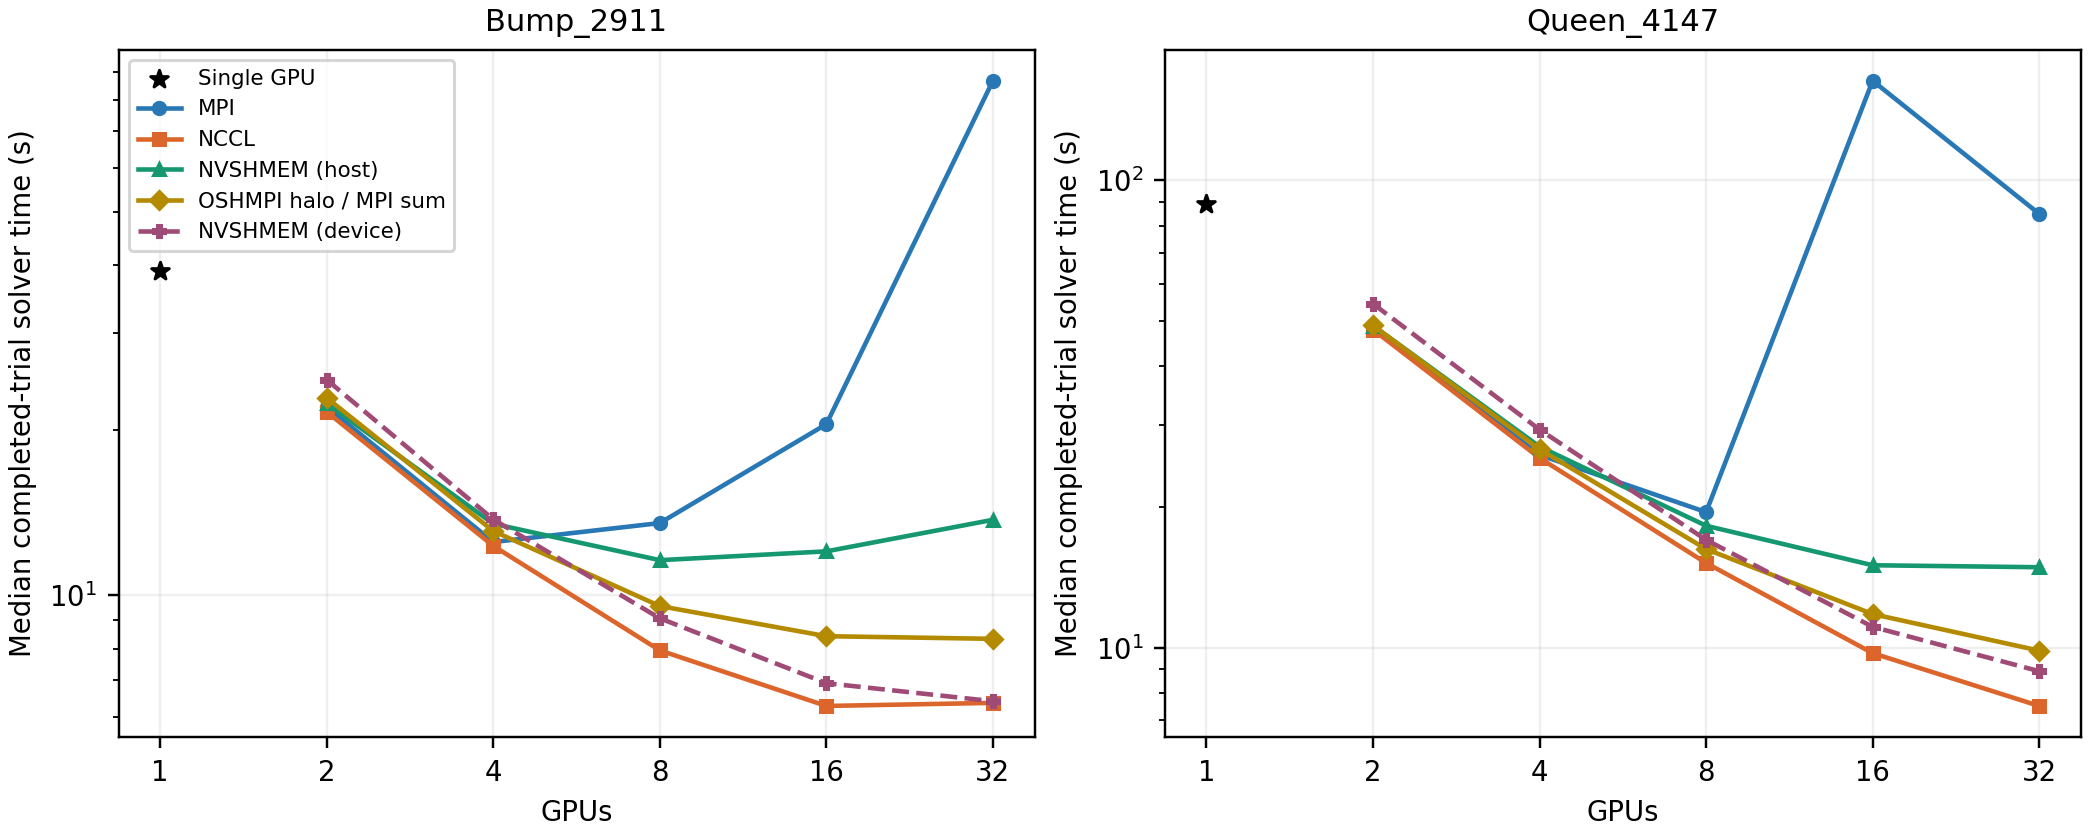
\includegraphics[width=\textwidth]{figures/results/acg-backend-median.png}
\caption{Median solver time over retained residual-valid completed trials for all native aCG paths. The device-NVSHMEM series changes solver organization as well as invocation. MPI's large-scale medians expose the slow mode that a fastest-trial curve would hide.}
\label{fig:m-acg-backend-median}
\end{figure}

\begin{table}[htbp]
\centering
\caption{OSHMPI-halo aCG results from the fastest residual-valid trial. Relative columns compare analytical throughput, not solver-time ratios.}
\label{tab:m-acg-oshmpi}
\footnotesize
\input{data/main-campaign/acg-oshmpi-table.tex}
\end{table}

\begin{figure}[htbp]
\centering
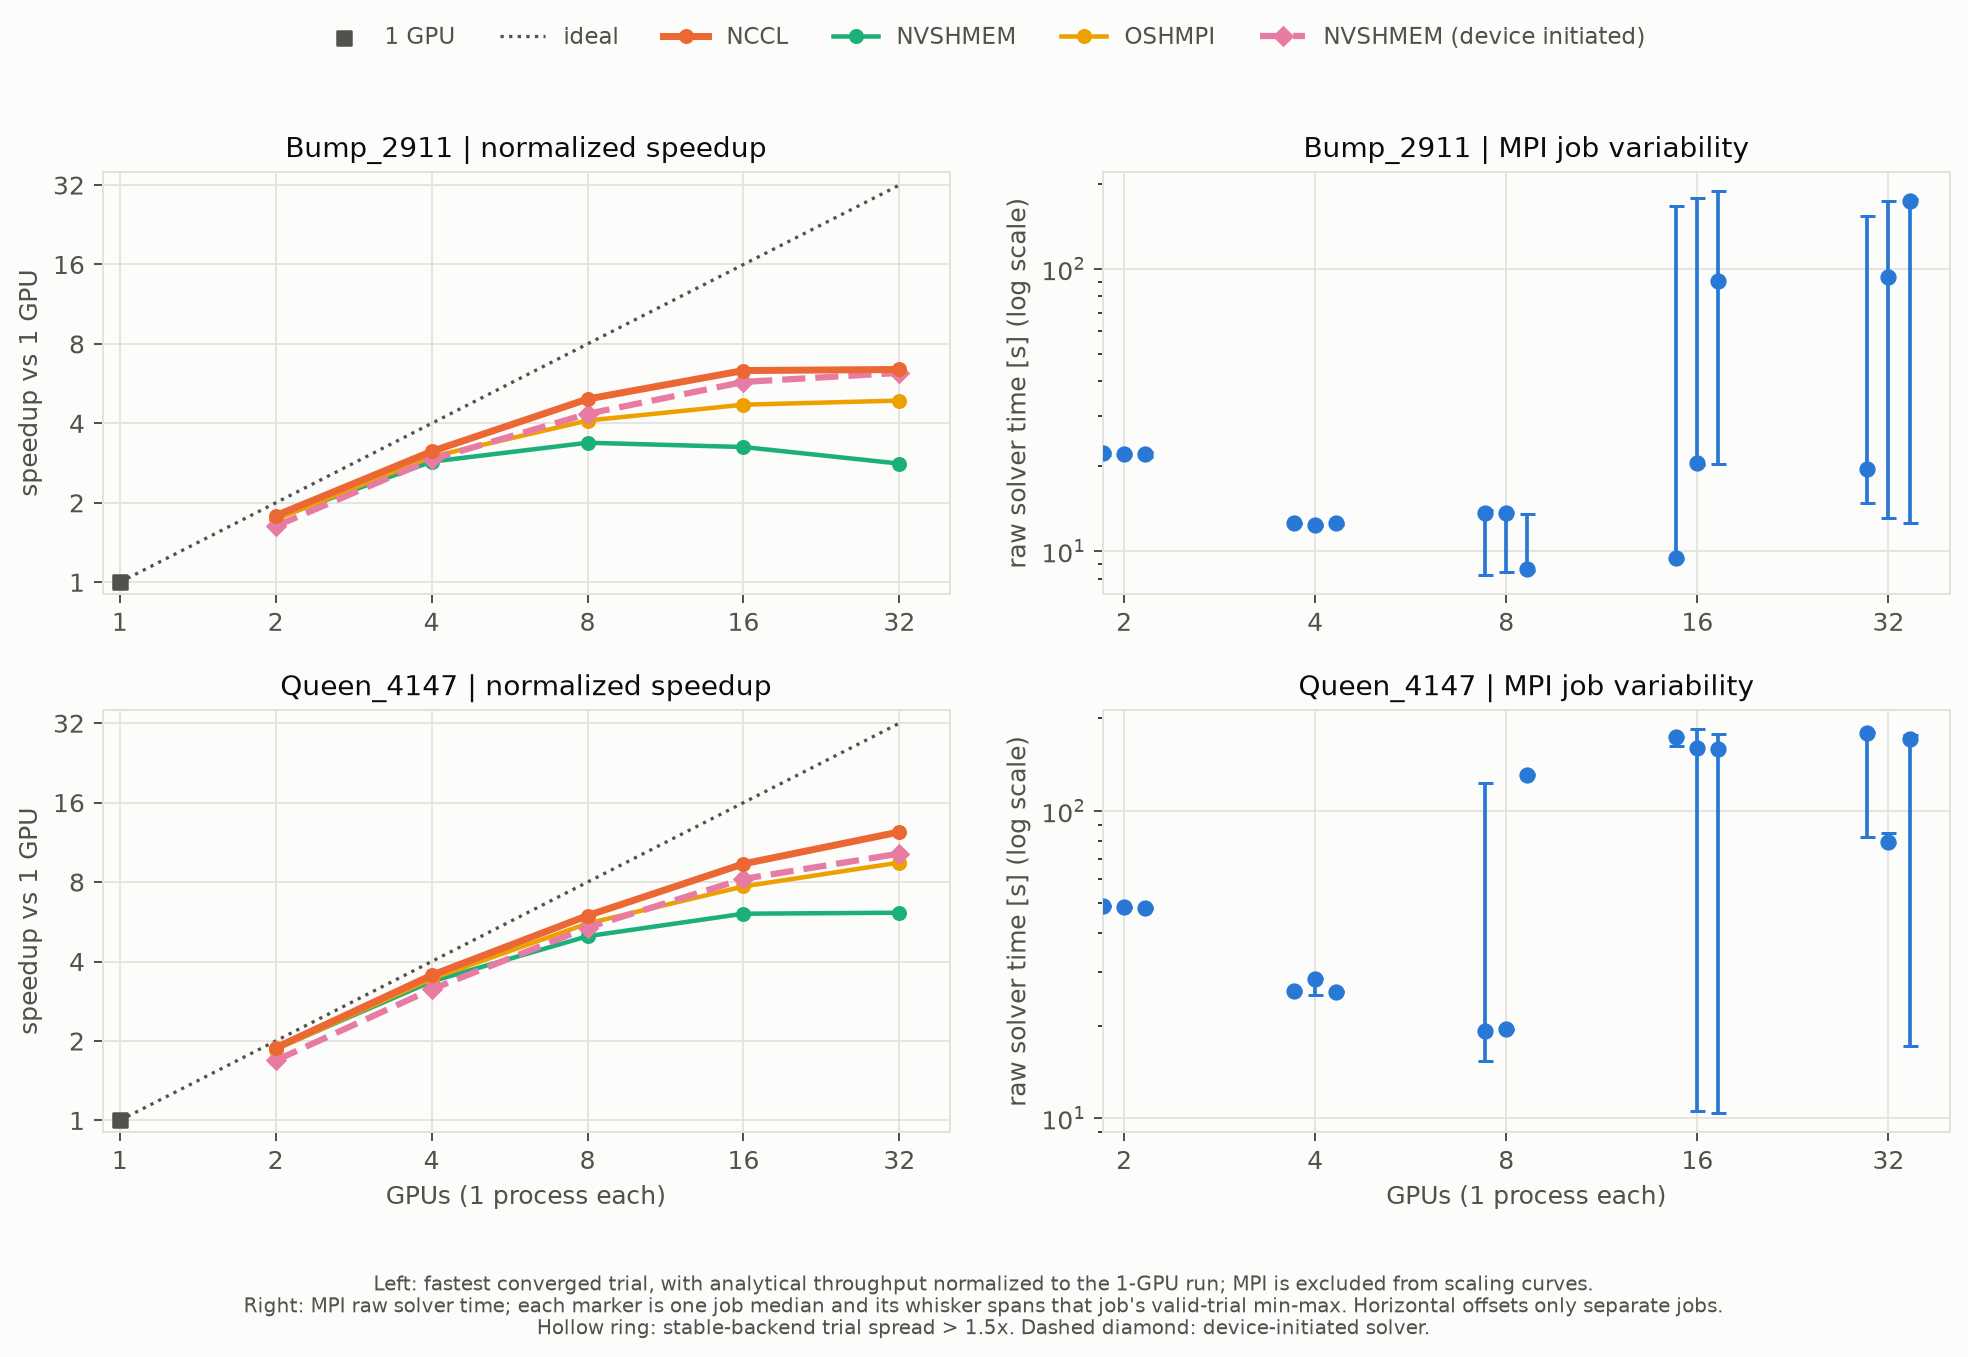
\includegraphics[width=\textwidth]{figures/results/acg-campaign-summary.png}
\caption{aCG scaling and variability. Left: analytical throughput of fastest-valid trials normalized to the one-GPU reference. Right: MPI solver time by allocation, with median markers and trial minimum--maximum ranges. The dashed device-NVSHMEM series changes solver organization as well as initiation.}
\label{fig:m-acg-scaling}
\end{figure}

Figure~\ref{fig:m-acg-scaling} separates the stable scaling trends from MPI variability. The monolithic NVSHMEM solver improves relative to blocking OSHMPI at larger process counts, although NCCL remains ahead in these work-normalized curves. This is consistent with reducing repeated host synchronization, but also reflects changed solver organization. Inter-node device requests still use the CPU proxy.

OSHMPI increasingly outperforms the host-NVSHMEM configuration. That result must be read with the application's disabled NCCL dispatch: it compares the installed native NVSHMEM reduction path, not the NCCL-dispatched path used by the default benchmark.

\subsection{Cross-Level Agreement for Scalar Reductions}

The most direct cross-level check pairs the operation actually executed rather than the communicator's name (Table~\ref{tab:m-acg-reduction-pairing}). Both the composite step and steady CG iteration perform two separate one-double global sums. The comparison uses half the composite reduction phase and compares it with the application's recorded cost per reduction.

\begin{table}[htbp]
\centering
\caption{Reduction pairings and remaining configuration differences.}
\label{tab:m-acg-reduction-pairing}
\footnotesize
\begin{tabularx}{\textwidth}{lYY}
\toprule
Composite path & Application path & Interpretation\\
\midrule
CUDA MPI & MPI scalar calls with OSHMPI halo & Avoids mixing the unstable MPI halo into the reference\\
CUDA NCCL & NCCL communicator & Same scalar collective interface\\
CUDA NVSHMEM & Host-NVSHMEM communicator & NCCL dispatch differs in the default archive\\
Direct OSHMPI & No matched archived scalar path & Benchmark stages to host; application reduces through MPI\\
\bottomrule
\end{tabularx}
\end{table}

\begin{figure}[htbp]
\centering
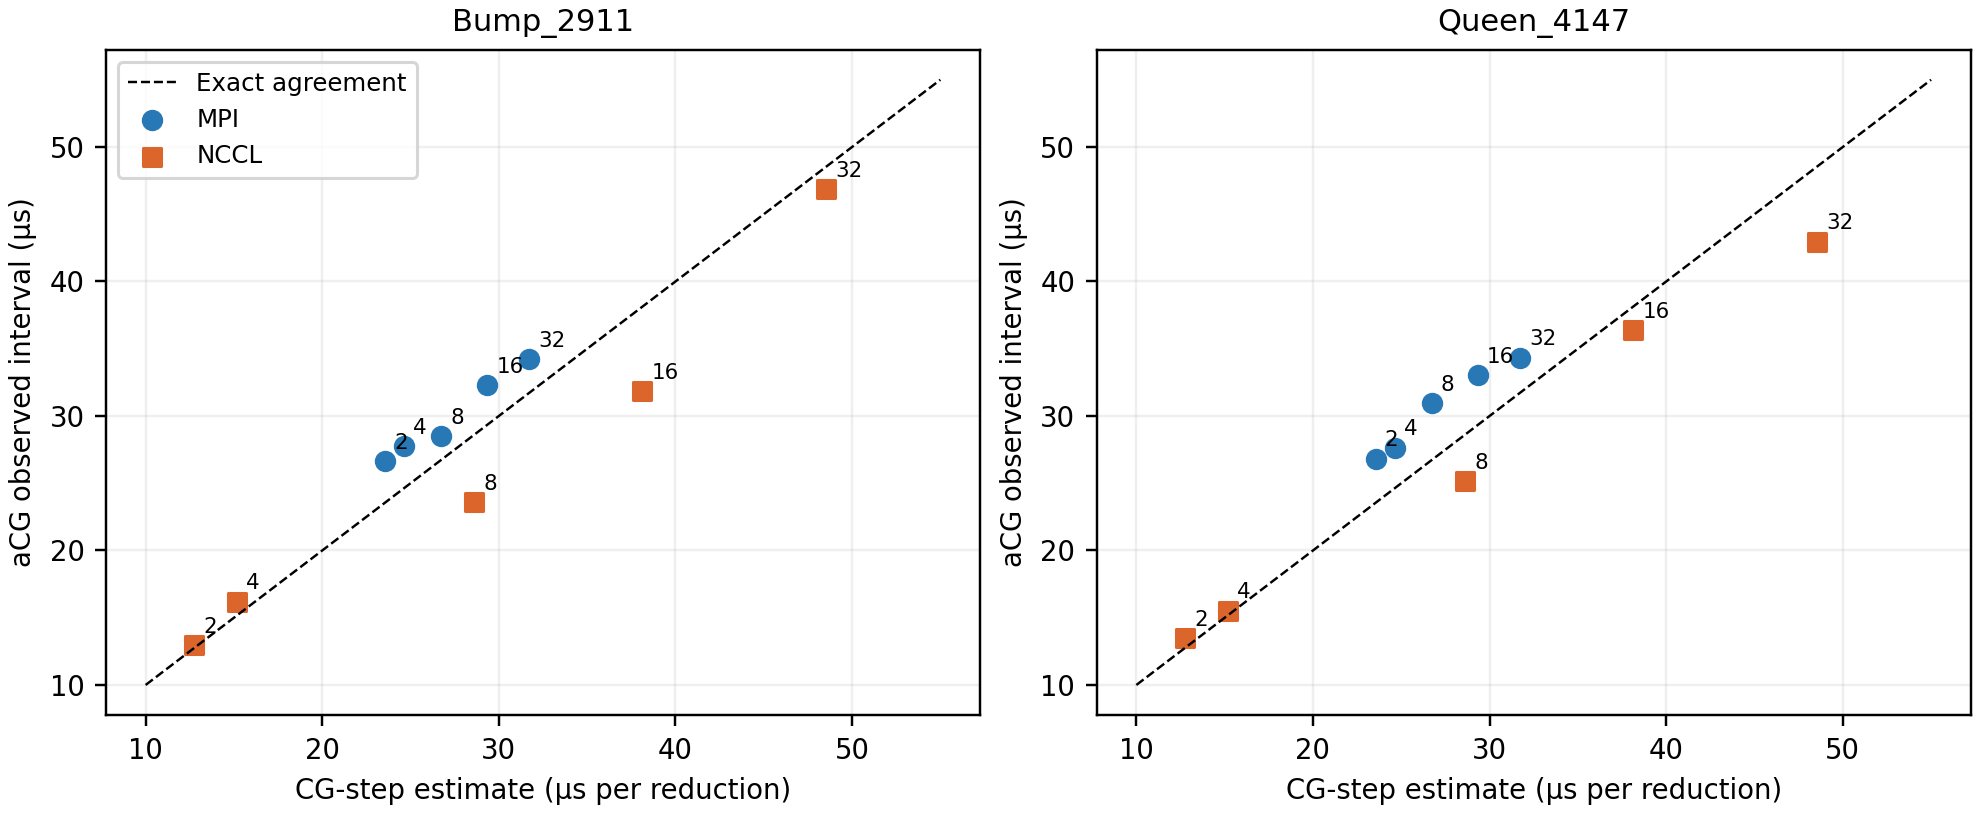
\includegraphics[width=\textwidth]{figures/results/acg-reduction-prediction.png}
\caption{One-double composite estimate versus aCG measurement. Point labels give GPU count. The dashed line is exact agreement; no model is fitted to these points. MPI observations come from the OSHMPI-halo solver.}
\label{fig:m-acg-reduction-prediction}
\end{figure}

\begin{table}[htbp]
\centering
\caption{Mean absolute percentage discrepancy over five measured rank counts, regenerated from the retained cross-level pairs.}
\label{tab:m-acg-reduction-correlation}
% Generated by tools/rebuild_main_evidence.py; include outside tabular.
\begin{tabular}{lrr}
\toprule
Reduction path & Bump\_2911 & Queen\_4147\\
\midrule
MPI & 9.2\% & 11.1\%\\
NCCL & 10.5\% & 7.8\%\\
\bottomrule
\end{tabular}

\end{table}

The mean discrepancies range from 7.8\% to 11.1\%. Individual cells can differ more: the NCCL Bump estimate is approximately 20\% high at eight and 16 GPUs. Figure~\ref{fig:m-acg-reduction-prediction} makes this distinction visible; a mean error is not an upper bound on every comparison. Because no model is fitted or held out and the application interval includes rank-arrival skew, the result establishes approximate scalar-cost agreement across the measured rank range, not general prediction accuracy or a numerical prediction of complete solver time.

The auxiliary configuration analysis reports that disabling NCCL dispatch materially changes NVSHMEM reduction time and gives matched errors of approximately 14--21\%. The matched per-trial arm is not present in the imported default JSON, so it is not plotted as an independently regenerated prediction. Repeating that control with explicit metadata would bring NVSHMEM to the same reproducibility level as the MPI/NCCL pairs. The separately recorded UCX-threshold control changes the composite MPI step by only approximately 2--3\%, which is too small to explain the much larger application variability.

\subsection{Irregular Peers and Overlap Change the Halo Question}

The regular halo and composite step do not reproduce aCG's exchange. The synthetic step has at most two fixed neighbors and a small structured payload. Table~\ref{tab:m-acg-halo-signatures} reconstructs the application signatures from the stored communication matrices, with element-to-byte conversion checked against the per-rank log totals. Bump reaches a mean of 10.8 outgoing neighbors at 32 GPUs, with as many as 17 on an individual rank. These asymmetric graphs are available as replay inputs in the reconciled archive. Nonblocking MPI and NCCL paths may progress while local SpMV executes, whereas the measured OSHMPI path completes before that work begins.

\begin{table}[htbp]
\centering
\caption{Application halo signatures reconstructed from the fixed sparse partitions. Volume is mean outgoing KiB per rank and exchange, excluding reductions.}
\label{tab:m-acg-halo-signatures}
\footnotesize
\input{data/main-campaign/halo-signature-table.tex}
\end{table}

The nominal halo timer cannot resolve this difference by itself. It measures only the wait at halo-end. For OSHMPI, communication has already completed in halo-begin, so a small halo column coexists with a substantial cost in \emph{other}. Dividing the full payload by that residual wait produces an apparent bandwidth, not a physical transfer rate. A comparison of isolated halo latency with this column would therefore compare different intervals.

Auxiliary attempts to replace global barriers with neighbor flags or to split begin/end without deferring completion did not improve total solver time. They show why a change in timer placement is insufficient to create overlap. A useful next comparison must retain the same peer graph and measure submission, progress, completion, and exposed wait around independent local work.

These differences explain why the composite winner need not be the solver winner. The benchmark's scalar completion contract and the application's reduction primitive differ, while halo structure and overlap also change. The current evidence cannot assign the ranking reversal to any one of these factors.

\subsection{Convergence and MPI Variability}

All 507 retained completed logs meet the recorded relative residual criterion, including 90 OSHMPI trials. This validates the recorded numerical outcome of those runs; it does not imply that every attempted run completed or that floating-point reduction order leaves iteration counts unchanged. Both total time and executed work are retained so that convergence differences remain visible.

MPI shows a separate performance-variability problem. Its halo and subsequent allreduce intervals grow together in slow runs, whereas the OSHMPI-halo solver uses the same MPI scalar interface with much more stable reduction timings. The contrast implicates the surrounding exchange and rank-arrival behavior, but does not isolate a particular UCX state or a single progress mechanism.

Large variations also occur among trials within one allocation, as Figure~\ref{fig:m-acg-scaling} shows. Node selection alone is therefore insufficient to explain the effect. Valid solutions can coexist with timing decompositions whose overlapping event regions are unsuitable for phase attribution. The chapter consequently reports MPI allocation ranges and avoids presenting its rare fastest run as a representative scaling curve. The irregular-halo replay is intended to test whether the behavior can be reproduced outside the complete solver.

\subsection{Supporting CUDA--SYCL Evidence}

The separate comparison report gives the median solver-time ratios in Table~\ref{tab:m-sycl-control}. These correspond to approximately 17--45\% additional time for the SYCL implementation. Both sides use medians, although this report is distinct from the main fastest-trial campaign.

\begin{table}[htbp]
\centering
\caption{Reported SYCL/CUDA median solver-time ratio for Bump\_2911. Correctness classification of the CUDA report requires reprocessing as described in Section~\ref{sec:acg-method}.}
\label{tab:m-sycl-control}
\begin{tabular}{rr}
\toprule
GPUs & SYCL/CUDA time\\
\midrule
1 & $1.336\times$\\
4 & $1.400\times$\\
8 & $1.446\times$\\
16 & $1.170\times$\\
\bottomrule
\end{tabular}
\end{table}

The ratio narrows at 16 GPUs, but the timing summaries alone do not establish why. Computation, host orchestration, and communication scaling all change their contribution to runtime. The communication-free composite controls independently show that a CUDA--SYCL implementation gap can exist without inter-rank transfers. Together, these observations motivate a matched implementation comparison with consistent correctness parsing and phase boundaries; they do not isolate a compiler penalty or establish cross-vendor performance portability.
